% Options for packages loaded elsewhere
\PassOptionsToPackage{unicode}{hyperref}
\PassOptionsToPackage{hyphens}{url}
%
\documentclass[
]{book}
\usepackage{lmodern}
\usepackage{amssymb,amsmath}
\usepackage{ifxetex,ifluatex}
\ifnum 0\ifxetex 1\fi\ifluatex 1\fi=0 % if pdftex
  \usepackage[T1]{fontenc}
  \usepackage[utf8]{inputenc}
  \usepackage{textcomp} % provide euro and other symbols
\else % if luatex or xetex
  \usepackage{unicode-math}
  \defaultfontfeatures{Scale=MatchLowercase}
  \defaultfontfeatures[\rmfamily]{Ligatures=TeX,Scale=1}
\fi
% Use upquote if available, for straight quotes in verbatim environments
\IfFileExists{upquote.sty}{\usepackage{upquote}}{}
\IfFileExists{microtype.sty}{% use microtype if available
  \usepackage[]{microtype}
  \UseMicrotypeSet[protrusion]{basicmath} % disable protrusion for tt fonts
}{}
\makeatletter
\@ifundefined{KOMAClassName}{% if non-KOMA class
  \IfFileExists{parskip.sty}{%
    \usepackage{parskip}
  }{% else
    \setlength{\parindent}{0pt}
    \setlength{\parskip}{6pt plus 2pt minus 1pt}}
}{% if KOMA class
  \KOMAoptions{parskip=half}}
\makeatother
\usepackage{xcolor}
\IfFileExists{xurl.sty}{\usepackage{xurl}}{} % add URL line breaks if available
\IfFileExists{bookmark.sty}{\usepackage{bookmark}}{\usepackage{hyperref}}
\hypersetup{
  pdftitle={Screen Pixel Ruler {[}master{]}},
  pdfauthor={Stewart Cossey},
  hidelinks,
  pdfcreator={LaTeX via pandoc}}
\urlstyle{same} % disable monospaced font for URLs
\usepackage{color}
\usepackage{fancyvrb}
\newcommand{\VerbBar}{|}
\newcommand{\VERB}{\Verb[commandchars=\\\{\}]}
\DefineVerbatimEnvironment{Highlighting}{Verbatim}{commandchars=\\\{\}}
% Add ',fontsize=\small' for more characters per line
\usepackage{framed}
\definecolor{shadecolor}{RGB}{248,248,248}
\newenvironment{Shaded}{\begin{snugshade}}{\end{snugshade}}
\newcommand{\AlertTok}[1]{\textcolor[rgb]{0.94,0.16,0.16}{#1}}
\newcommand{\AnnotationTok}[1]{\textcolor[rgb]{0.56,0.35,0.01}{\textbf{\textit{#1}}}}
\newcommand{\AttributeTok}[1]{\textcolor[rgb]{0.77,0.63,0.00}{#1}}
\newcommand{\BaseNTok}[1]{\textcolor[rgb]{0.00,0.00,0.81}{#1}}
\newcommand{\BuiltInTok}[1]{#1}
\newcommand{\CharTok}[1]{\textcolor[rgb]{0.31,0.60,0.02}{#1}}
\newcommand{\CommentTok}[1]{\textcolor[rgb]{0.56,0.35,0.01}{\textit{#1}}}
\newcommand{\CommentVarTok}[1]{\textcolor[rgb]{0.56,0.35,0.01}{\textbf{\textit{#1}}}}
\newcommand{\ConstantTok}[1]{\textcolor[rgb]{0.00,0.00,0.00}{#1}}
\newcommand{\ControlFlowTok}[1]{\textcolor[rgb]{0.13,0.29,0.53}{\textbf{#1}}}
\newcommand{\DataTypeTok}[1]{\textcolor[rgb]{0.13,0.29,0.53}{#1}}
\newcommand{\DecValTok}[1]{\textcolor[rgb]{0.00,0.00,0.81}{#1}}
\newcommand{\DocumentationTok}[1]{\textcolor[rgb]{0.56,0.35,0.01}{\textbf{\textit{#1}}}}
\newcommand{\ErrorTok}[1]{\textcolor[rgb]{0.64,0.00,0.00}{\textbf{#1}}}
\newcommand{\ExtensionTok}[1]{#1}
\newcommand{\FloatTok}[1]{\textcolor[rgb]{0.00,0.00,0.81}{#1}}
\newcommand{\FunctionTok}[1]{\textcolor[rgb]{0.00,0.00,0.00}{#1}}
\newcommand{\ImportTok}[1]{#1}
\newcommand{\InformationTok}[1]{\textcolor[rgb]{0.56,0.35,0.01}{\textbf{\textit{#1}}}}
\newcommand{\KeywordTok}[1]{\textcolor[rgb]{0.13,0.29,0.53}{\textbf{#1}}}
\newcommand{\NormalTok}[1]{#1}
\newcommand{\OperatorTok}[1]{\textcolor[rgb]{0.81,0.36,0.00}{\textbf{#1}}}
\newcommand{\OtherTok}[1]{\textcolor[rgb]{0.56,0.35,0.01}{#1}}
\newcommand{\PreprocessorTok}[1]{\textcolor[rgb]{0.56,0.35,0.01}{\textit{#1}}}
\newcommand{\RegionMarkerTok}[1]{#1}
\newcommand{\SpecialCharTok}[1]{\textcolor[rgb]{0.00,0.00,0.00}{#1}}
\newcommand{\SpecialStringTok}[1]{\textcolor[rgb]{0.31,0.60,0.02}{#1}}
\newcommand{\StringTok}[1]{\textcolor[rgb]{0.31,0.60,0.02}{#1}}
\newcommand{\VariableTok}[1]{\textcolor[rgb]{0.00,0.00,0.00}{#1}}
\newcommand{\VerbatimStringTok}[1]{\textcolor[rgb]{0.31,0.60,0.02}{#1}}
\newcommand{\WarningTok}[1]{\textcolor[rgb]{0.56,0.35,0.01}{\textbf{\textit{#1}}}}
\usepackage{longtable,booktabs}
% Correct order of tables after \paragraph or \subparagraph
\usepackage{etoolbox}
\makeatletter
\patchcmd\longtable{\par}{\if@noskipsec\mbox{}\fi\par}{}{}
\makeatother
% Allow footnotes in longtable head/foot
\IfFileExists{footnotehyper.sty}{\usepackage{footnotehyper}}{\usepackage{footnote}}
\makesavenoteenv{longtable}
\usepackage{graphicx,grffile}
\makeatletter
\def\maxwidth{\ifdim\Gin@nat@width>\linewidth\linewidth\else\Gin@nat@width\fi}
\def\maxheight{\ifdim\Gin@nat@height>\textheight\textheight\else\Gin@nat@height\fi}
\makeatother
% Scale images if necessary, so that they will not overflow the page
% margins by default, and it is still possible to overwrite the defaults
% using explicit options in \includegraphics[width, height, ...]{}
\setkeys{Gin}{width=\maxwidth,height=\maxheight,keepaspectratio}
% Set default figure placement to htbp
\makeatletter
\def\fps@figure{htbp}
\makeatother
\setlength{\emergencystretch}{3em} % prevent overfull lines
\providecommand{\tightlist}{%
  \setlength{\itemsep}{0pt}\setlength{\parskip}{0pt}}
\setcounter{secnumdepth}{-\maxdimen} % remove section numbering
\usepackage{booktabs}
\usepackage{amsthm}
\makeatletter
\def\thm@space@setup{%
  \thm@preskip=8pt plus 2pt minus 4pt
  \thm@postskip=\thm@preskip
}
\makeatother
\usepackage[]{natbib}
\bibliographystyle{plainnat}

\title{Screen Pixel Ruler {[}master{]}}
\author{Stewart Cossey}
\date{2021-12-06}

\begin{document}
\maketitle

{
\setcounter{tocdepth}{1}
\tableofcontents
}
\hypertarget{overview}{%
\chapter{Overview}\label{overview}}

Screen Pixel Ruler is a on screen ruler that can assist in measuring elements from web pages, documents or software which does not implement a native ruler.
Based on .NET Core 3.1 and inspired by MioPlanet PixelRuler, this software is supported on Windows 7 and higher.

\hypertarget{features}{%
\section{Features}\label{features}}

\begin{itemize}
\tightlist
\item
  Global hotkeys to trigger functionality when other software is in focus.
\item
  Rotatable vertical or horizontal ruler. \texttt{Ctrl\ +\ Shift\ +\ Alt\ +\ R}
\item
  Customizable ruler themes.
\item
  Freezable position. \texttt{Ctrl\ +\ Shift\ +\ Alt\ +\ F}
\item
  Guideline system that can lock the mouse cursor horizontally or vertically
\item
  Position 0 of the ruler to the current cursor location. \texttt{Ctrl\ +\ Shift\ +\ Alt\ +\ S}
\end{itemize}

\begin{quote}
A list of all shorcuts can be found \protect\hyperlink{keyboard}{here}.
\end{quote}

\hypertarget{installation}{%
\section{Installation}\label{installation}}

Screen Pixel Ruler can be installed from either the \href{https://github.com/Cossey/ScreenPixelRuler2/releases}{Installer} or via \href{https://chocolatey.org}{Chocolatey Package Management} by running the command \texttt{choco\ install\ screenpixelruler}.
Both the installer and package will install the .NET Core 3.1 runtime if it is not present.

\hypertarget{ui}{%
\chapter{User Interface}\label{ui}}

The user interface consists of a single ruler that can be displayed either horizontally or vertically.

\begin{figure}
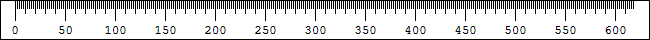
\includegraphics[width=1\linewidth]{images/ruler} \caption{The Ruler user interface.}\label{fig:unnamed-chunk-1}
\end{figure}

Pressing the secondary mouse button on the ruler will display a context menu called the \emph{Ruler Menu}.
The secondary button is usually the right mouse button.

The ruler can be rotated using the \texttt{Ctrl\ +\ Shift\ +\ Alt\ +\ R} key combination or by the \emph{Rotate} menu item in the \emph{Ruler Menu}.

\begin{quote}
It is not possible to have both a vertical and a horizontal ruler displayed at the same time.
\end{quote}

\hypertarget{guidelines}{%
\chapter{Guidelines}\label{guidelines}}

Guidelines allow you to mark specific points on the ruler.

\hypertarget{adding-and-removing-guidelines}{%
\section{Adding and Removing Guidelines}\label{adding-and-removing-guidelines}}

You can add and remove guidelines by using the Ruler Menu \textgreater{} Guidelines submenu.
Adding a guideline will add a new guideline at the cursor position on the ruler.

\hypertarget{clearing-guidelines}{%
\section{Clearing Guidelines}\label{clearing-guidelines}}

\hypertarget{importing-and-exporting-guidelines}{%
\section{Importing and Exporting Guidelines}\label{importing-and-exporting-guidelines}}

\hypertarget{keyboard}{%
\chapter{Global Shortcuts}\label{keyboard}}

\begin{quote}
These shortcuts can be used even when the Screen Pixel Ruler is not focused.
\end{quote}

\begin{longtable}[]{@{}ll@{}}
\toprule
\begin{minipage}[b]{0.27\columnwidth}\raggedright
Keystroke\strut
\end{minipage} & \begin{minipage}[b]{0.68\columnwidth}\raggedright
Function\strut
\end{minipage}\tabularnewline
\midrule
\endhead
\begin{minipage}[t]{0.27\columnwidth}\raggedright
Ctrl + Shift + Alt + R\strut
\end{minipage} & \begin{minipage}[t]{0.68\columnwidth}\raggedright
Change ruler rotation.\strut
\end{minipage}\tabularnewline
\begin{minipage}[t]{0.27\columnwidth}\raggedright
Ctrl + Shift + Alt + E\strut
\end{minipage} & \begin{minipage}[t]{0.68\columnwidth}\raggedright
Flip ruler notch direction.\strut
\end{minipage}\tabularnewline
\begin{minipage}[t]{0.27\columnwidth}\raggedright
Ctrl + Shift + Alt + F\strut
\end{minipage} & \begin{minipage}[t]{0.68\columnwidth}\raggedright
Freeze the position marker on the ruler.\strut
\end{minipage}\tabularnewline
\begin{minipage}[t]{0.27\columnwidth}\raggedright
Ctrl + Shift + Alt + S\strut
\end{minipage} & \begin{minipage}[t]{0.68\columnwidth}\raggedright
Move position 0 of the ruler to the current mouse position.\strut
\end{minipage}\tabularnewline
\begin{minipage}[t]{0.27\columnwidth}\raggedright
Ctrl + Shift + Alt + X\strut
\end{minipage} & \begin{minipage}[t]{0.68\columnwidth}\raggedright
Exit Screen Pixel Ruler 2.\strut
\end{minipage}\tabularnewline
\begin{minipage}[t]{0.27\columnwidth}\raggedright
Ctrl + Shift + Alt + A\strut
\end{minipage} & \begin{minipage}[t]{0.68\columnwidth}\raggedright
Add Guideline at current position on the ruler.\strut
\end{minipage}\tabularnewline
\begin{minipage}[t]{0.27\columnwidth}\raggedright
Ctrl + Shift + Alt + D\strut
\end{minipage} & \begin{minipage}[t]{0.68\columnwidth}\raggedright
Delete nearest Guideline from current position on the ruler.\strut
\end{minipage}\tabularnewline
\begin{minipage}[t]{0.27\columnwidth}\raggedright
Ctrl + Shift + Alt + G\strut
\end{minipage} & \begin{minipage}[t]{0.68\columnwidth}\raggedright
Lock mouse position to nearest Guideline.\strut
\end{minipage}\tabularnewline
\bottomrule
\end{longtable}

\hypertarget{config}{%
\chapter{Configuration}\label{config}}

You can access the configuration by right clicking the ruler and selecting \emph{Options}.
This will then display the \emph{Options window} where you can change the configuration.

\begin{figure}
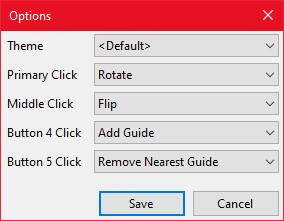
\includegraphics[width=1\linewidth]{images/options} \caption{The options window.}\label{fig:unnamed-chunk-2}
\end{figure}

\hypertarget{options}{%
\section{Options}\label{options}}

\hypertarget{theme}{%
\subsection{Theme}\label{theme}}

Allows you to change the \protect\hyperlink{themes}{theme} of the ruler.

\hypertarget{primary-click-middle-click-button-4-click-button-5-click}{%
\subsection{Primary Click, Middle Click, Button 4 Click, Button 5 Click}\label{primary-click-middle-click-button-4-click-button-5-click}}

Allows you to assign mouse button clicking the ruler to specific functionality.
Pressing and holding the primary click will allow you to move the ruler.

\begin{quote}
The primary click is determined by the \emph{Select your primary button} option in the \emph{Mouse Settings} on Microsoft Windows.
\end{quote}

\hypertarget{location}{%
\section{Location}\label{location}}

Configuration is stored in two locations depending on if you installed from the installer or from the chocolatey package.

Installer: \%appdata\%\textbackslash screenpixelruler\textbackslash app.cfg\\
Chocolatey: \%chocolateyinstall\%\textbackslash lib\textbackslash screenpixelruler\textbackslash tools\textbackslash app.cfg

\hypertarget{themes}{%
\chapter{Themes}\label{themes}}

Themes can change the ruler colour, size or even the interval of the hatch marks.
Screen Pixel Ruler comes with some supplied themes.

\hypertarget{supplied-themes}{%
\section{Supplied Themes}\label{supplied-themes}}

\hypertarget{default}{%
\subsection{Default}\label{default}}

A simple black and white theme with a thin ruler. Great contrasting for easy visibility.

\hypertarget{panda}{%
\subsection{Panda}\label{panda}}

A dark themed and large ruler.

\hypertarget{mioplanet-pixelruler}{%
\subsection{MioPlanet PixelRuler}\label{mioplanet-pixelruler}}

A blue ruled designed to mimic the MioPlanet PixelRuler software.

\hypertarget{white-chocolate}{%
\subsection{White Chocolate}\label{white-chocolate}}

A white on brown coloured theme.

\hypertarget{location-1}{%
\section{Location}\label{location-1}}

Themes are stored in the two locations, depending on if you installed from the installer or from the chocolatey package.

Installer: \%appdata\%\textbackslash screenpixelruler\\
Chocolatey: \%chocolateyinstall\%\textbackslash lib\textbackslash screenpixelruler\textbackslash tools

\hypertarget{creating-a-theme}{%
\section{Creating a Theme}\label{creating-a-theme}}

You can create your own themes for Screen Pixel Ruler.
Themes have a \texttt{thm} file extension and are writtem in \href{https://yaml.org}{yaml}.

\hypertarget{objects}{%
\subsection{Objects}\label{objects}}

A string of text.

Either \texttt{true} or \texttt{false}.

A decimal number like \texttt{1.0} or \texttt{1.5}.

A number like \texttt{1} or \texttt{15}.

An array of objects.

A colour value.
Supported input types are:
- \texttt{\textquotesingle{}\#RRGGBB\textquotesingle{}} Hex/HTML Colour
- \texttt{RRR,\ GGG,\ BBB} Decimal (0-255)
- \texttt{ColorName} Name

An array of either one (\texttt{{[}\ \textless{}colour\textgreater{}\ {]}}) or two colour values (\texttt{{[}\ \textless{}colour\textgreater{},\ \textless{}colour\textgreater{}\ {]}}).
If two colours are provided then the colour will be a gradient of both colours.

\begin{quote}
For a list of colour names see the \href{https://docs.microsoft.com/en-us/dotnet/api/system.drawing.knowncolor?view=netcore-3.1}{KnownColor Enum} reference.
\end{quote}

\hypertarget{file-format}{%
\subsection{File Format}\label{file-format}}

\hypertarget{fields}{%
\subsubsection{Fields}\label{fields}}

\begin{Shaded}
\begin{Highlighting}[]
\AttributeTok{Name <string> *The name of the theme.*}
\AttributeTok{Cursor *Cursor themeing.*}
\AttributeTok{  Line <colour> *The cursor line colour.*}
\AttributeTok{  Font *The font used for the cursor.*}
\AttributeTok{    Family <string> *The font family.*}
\AttributeTok{    Size <decimal> *The font size.*}
\AttributeTok{    Bold <boolean> *Whether the font is bold.*}
\AttributeTok{    Italic <boolean> *Whether the font is italicised.*}
\AttributeTok{    Underline <boolean> *Whether the font is underlined.*}
\AttributeTok{    Strikeout <boolean> *Whether the font is striked out.*}
\AttributeTok{  Background <colours> *The background colours for the cursor.*}
\AttributeTok{  Frozen *The frozen colours for the cursor.*}
\AttributeTok{    Line <colour> *The frozen line colour.*}
\AttributeTok{    Font *The font used for the frozen cursor.*}
\AttributeTok{      Family <string> *The font family.*}
\AttributeTok{      Size <decimal> *The font size.*}
\AttributeTok{      Bold <boolean> *Whether the font is bold.*}
\AttributeTok{      Italic <boolean> *Whether the font is italicised.*}
\AttributeTok{      Underline <boolean> *Whether the font is underlined.*}
\AttributeTok{      Strikeout <boolean> *Whether the font is striked out.*}
\AttributeTok{    Background <colours> *The frozen background colours.*}
\AttributeTok{  Locked *The guideline locked colours for the cursor.*}
\AttributeTok{    Line <colour> *The locked line colour.*}
\AttributeTok{    Font *The font used for the locked cursor.*}
\AttributeTok{      Family <string> *The font family.*}
\AttributeTok{      Size <decimal> *The font size.*}
\AttributeTok{      Bold <boolean> *Whether the font is bold.*}
\AttributeTok{      Italic <boolean> *Whether the font is italicised.*}
\AttributeTok{      Underline <boolean> *Whether the font is underlined.*}
\AttributeTok{      Strikeout <boolean> *Whether the font is striked out.*}
\AttributeTok{    Background <colours> *The locked background colours.*}
\AttributeTok{Ruler *Ruler themeing.*}
\AttributeTok{  Size <number> *The size of the ruler in pixels.*}
\AttributeTok{  Background <colours> *The background colour for the ruler.*}
\AttributeTok{  Border}
\AttributeTok{    Colour <colour> *The border colour.*}
\AttributeTok{    Spacing <number> *The spacing between the border and the ruler.*}
\AttributeTok{  Marks *The hatch marks.*}
\AttributeTok{    Colour <colour> *The colour of the hatch marks.*}
\AttributeTok{    Size}
\AttributeTok{      Horizontal <number> *The size of the hatch marks when the ruler is horizontal.*}
\AttributeTok{      Vertical <number> *The size of the hatch marks when the ruler is vertical.*}
\AttributeTok{    Zero *The zero hatch mark.*}
\AttributeTok{        NumberVisible <boolean> *Whether the number zero is displayed.*}
\AttributeTok{        Size}
\AttributeTok{          Horizontal <number> *The size of the zero hatch mark when the ruler is horizontal.*}
\AttributeTok{          Vertical <number> *The size of the zero hatch mark when the ruler is vertical.*}
\AttributeTok{    Sizes <array> *The sizes of the hatch marks.*}
\AttributeTok{      Interval <number> *The interval of the hatch marks.*}
\AttributeTok{      Colour <colour> *The colour of the hatch marks.*}
\AttributeTok{      Size}
\AttributeTok{        Horizontal <number> *The size of the hatch marks when the ruler is horizontal.*}
\AttributeTok{        Vertical <number> *The size of the hatch marks when the ruler is vertical.*}
\AttributeTok{  Numbers *The numbers on the ruler.*}
\AttributeTok{    Padding}
\AttributeTok{      Horizontal <number> *The padding on the left and right of the numbers.*}
\AttributeTok{      Vertical <number> *The padding on the top and bottom of the numbers.*}
\AttributeTok{    Colour <colour> *The colour of the numbers.*}
\AttributeTok{    Font *The font used for the numbers.*}
\AttributeTok{      Family <string> *The font family.*}
\AttributeTok{      Size <decimal> *The font size.*}
\AttributeTok{      Bold <boolean> *Whether the font is bold.*}
\AttributeTok{      Italic <boolean> *Whether the font is italicised.*}
\AttributeTok{      Underline <boolean> *Whether the font is underlined.*}
\AttributeTok{      Strikeout <boolean> *Whether the font is striked out.*}
\AttributeTok{    Display}
\AttributeTok{      Interval <number> *The interval at which numbers should appear.*}
\AttributeTok{  Guidelines}
\AttributeTok{    Guideline *The guidelines.*}
\AttributeTok{      Colour <colour> *The colour of the guidelines.*}
\AttributeTok{      Size}
\AttributeTok{        Horizontal <number> *The size of the guidelines when the ruler is horizontal.*}
\AttributeTok{        Vertical <number> *The size of the guidelines when the ruler is vertical.*}
\AttributeTok{    Locked *The guideline locked onto.}
\AttributeTok{      Colour <colour> *The colour of the guideline that has been locked onto.*}
\AttributeTok{      Size}
\AttributeTok{        Horizontal <number> *The size of the guideline that has been locked onto when the ruler is horizontal.*}
\AttributeTok{        Vertical <number> *The size of the guideline that has been locked onto when the ruler is vertical.*}
\AttributeTok{    Nearest *The guideline nearest to the cursor.*}
\AttributeTok{      Colour <colour> *The colour of the nearest guideline.*}
\AttributeTok{      Size}
\AttributeTok{        Horizontal <number> *The size of the nearest guideline when the ruler is horizontal.*}
\AttributeTok{        Vertical <number> *The size of the nearest guideline when the ruler is vertical.*}
\end{Highlighting}
\end{Shaded}

\hypertarget{visual-guide}{%
\subsubsection{Visual Guide}\label{visual-guide}}

\begin{figure}
\centering
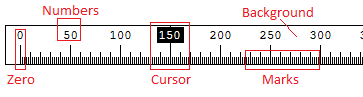
\includegraphics{images/ruler-theme.png}
\caption{\label{fig:unnamed-chunk-3}The Ruler user interface with theme elements highlighted.}
\end{figure}

\emph{Zero} is the \emph{Zero Mark} which is explained further below.

\emph{Numbers} are configured in \texttt{Ruler\ →\ Number} secion.
The \texttt{Ruler\ →\ Number\ →\ Display\ →\ Interval} determines how often the numbers appear.
An interval of \texttt{50} means that numbers will appear at the 50th, 100th, 150th, etc hatch marks.
The other properties under \texttt{Ruler\ →\ Number} determine the font, colour and size of the numbers.

\emph{Cursor} is the position of the mouse cursor on screen.
Fruther explaination below.

\emph{Background} is the background colour of the ruler.
This is set at \texttt{Ruler\ →\ Background} and can be a single colour or a gradient when two colours are provided.

\begin{figure}
\centering
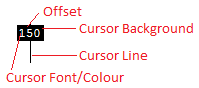
\includegraphics{images/ruler-cursor.png}
\caption{\label{fig:unnamed-chunk-4}The cursor that appears in the ruler.}
\end{figure}

The above options are all configured in the \texttt{Ruler\ →\ Cursor} section.

\begin{figure}
\centering
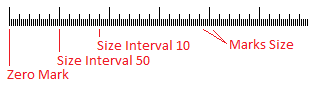
\includegraphics{images/ruler-hashmarks.png}
\caption{\label{fig:unnamed-chunk-5}The ruler hatch marks.}
\end{figure}

\emph{Zero Mark} hatch mark is provided by the \texttt{Ruler\ →\ Marks\ →\ Zero\ →\ Size} property.
You can also set the \texttt{Ruler\ →\ Marks\ →\ Zero\ →\ NumberVisible} property to \texttt{false} to omit the 0 number.

\emph{Size interval 10} and \emph{Size Interval 50} hatch marks are provided by the \texttt{Ruler\ →\ Marks\ →\ Sizes} array.
The 50 pixel interval hatch mark:

\begin{Shaded}
\begin{Highlighting}[]
\CommentTok{...}
\CommentTok{  Marks:}
\CommentTok{    Sizes:}
\CommentTok{      - Interval: 50}
\CommentTok{        Colour: #000000}
\CommentTok{        Size:}
\CommentTok{          Horizontal: 20}
\CommentTok{          Vertical: 40}
\CommentTok{...}
\end{Highlighting}
\end{Shaded}

\emph{Marks Size} hatch marks are provided by the \texttt{Ruler\ →\ Marks\ →\ Size} properties.
The colour is provided by the \texttt{Ruler\ →\ Marks\ →\ Colour} property.

\hypertarget{default-values}{%
\subsubsection{Default Values}\label{default-values}}

Font:
Family: Courier New
Size: 9
Bold: false
Italic: false
Underline: false
Strikeout: false

Cursor → Locked:
Cursor → Frozen

Cursor → Frozen:
Cursor

\end{document}
